
% \subsection{INSTITUTIONAL SHIFTS AND STRUCTURES}
\subsection{制度变迁研究框架}\label{results-1}

\begin{figure*}[!t]
	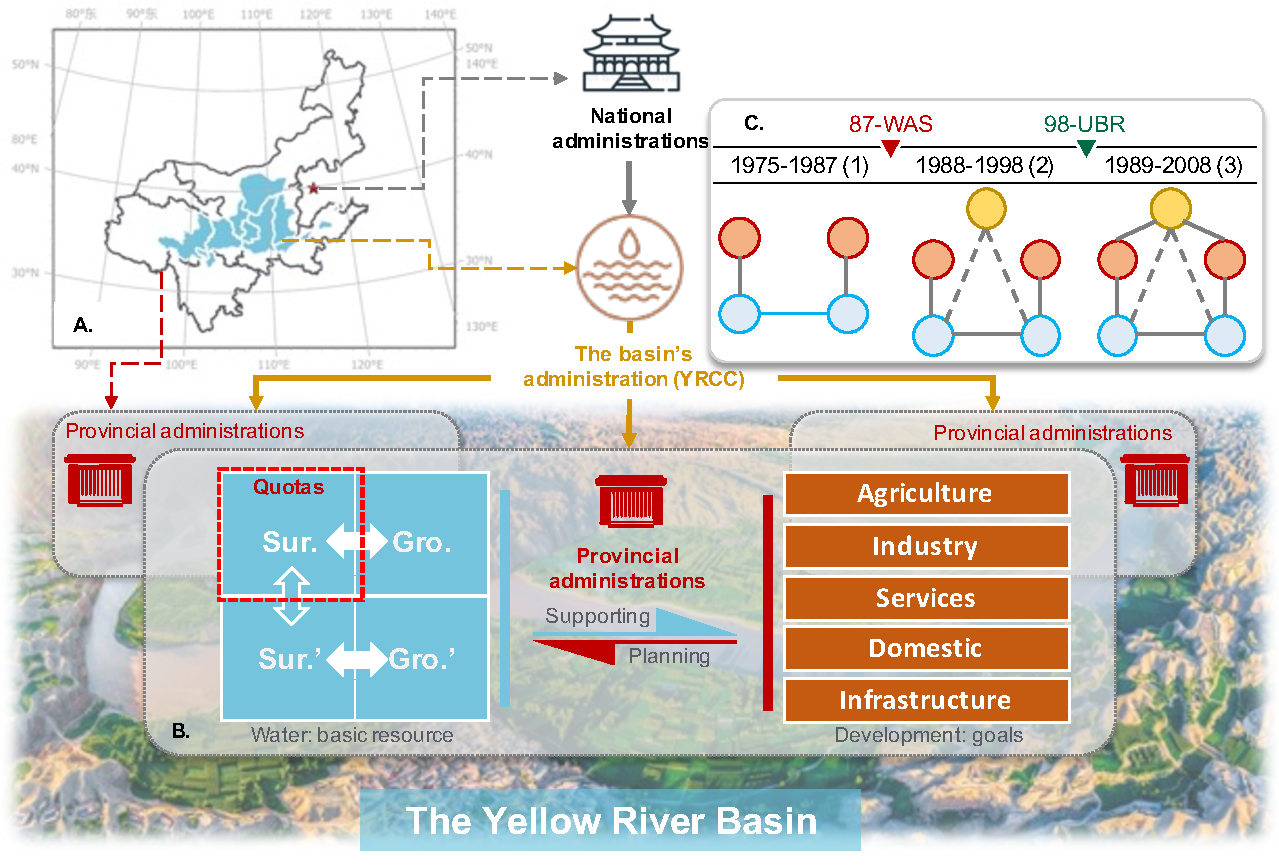
\includegraphics[width=\linewidth]{img/ch5/diagram.pdf}
	\caption[黄河流域社会经济制度变迁及其结构]{
		% 黄河流域的制度变迁与经济社会结构差异。
		黄河流域社会经济制度变迁及其结构。
		\textbf{A.} 长江流域跨越$10$个省(地区),其中$8$个对长江流域水资源的依赖程度较高。
		% (see \textit{\nameref{secS1}} Table~\ref{tab:quota})。
		国家行政部门是发布水治理政策的最终权力机构,这些政策通常由流域一级机构黄河水利委员会和各省级机构执行。
		\textbf{B.} 省级行政机关是主要的利益相关者。自87-WAS以来,由于黄河地表水的抽取受到特定配额的限制,各利益相关者规划和利用水资源进行发展。然而,自然水文过程是相互联系的。虽然这些机构主要关注地表水(Sur),但它也可能影响内部的地下水(Gro)或外部的水资源(Sur')。通过系统的社会水文过程在YRB。黄河水利委员会只监控当时的取水情况。
		\textbf{C.} 制度变迁和随之而来的结构变化
		% (details in \textit{\nameref{secS1}})
		(1) 1979 - 1987年间,各利益相关方(红圈表示)从连接的生态单元(黄河河段,蓝圈表示)自由获取水资源。
		(2) 1987-WAS后,黄河流域控制中心(黄圈)以用水定额监测河段(点线连接)。
		(3)自98-UBR以来,利益相关者必须向YRCC(红黄圈之间的连接)申请用水许可证。
	}\label{fig:structure}
\end{figure*}

% 制度变动综述
1987年(87-WAS)和1998年(98-UBR) YRB的制度转变是YRB水治理实践中限制用水的两个被广泛认可的里程碑。
% (\textit{\nameref{sec:yrb}} and \textit{\nameref{secS1}}).
在87-WAS之前,利益相关者(黄河流域的省份)可以自由使用黄河的水资源进行开发,但淡水需求和可用性之间存在地理和时间差异。
1987年以前,长江水利枢纽与各省在用水方面没有联系,各省可以直接与黄河河段相连(图~\ref{fig:structure}~C)。
在87-WAS中,为缩小水资源亏缺,国家主管部门在87-WAS中提出在YR流域10个省(或地区)之间分配特定的水资源配额(表~\ref{tab:quota})。
同时,根据国家部委发布的87-WAS文件中提取的信息,YRCC开始报告各个河段的用水情况。
由于这是长江流域水利枢纽的责任首次涉及水资源利用,这在长江流域水利枢纽与生态节点之间引入了新的联系(图~\ref{fig:structure}~C)。
然而,备受争议的87-WAS并没有解决流量枯竭问题。
1998年,制定了另一项战略(98-UBR),以加强YRCC在综合管理用水方面的责任。
来自98-UBR文件的信息表明,各省不得不将其年度用水许可证计划应用于YRCC,而不是直接使用黄河水。
因此,YRCC自1998年以来一直与各省联系在一起(图~\ref{fig:structure}~C)。
因此,两次制度转换重塑了,形成了三个由社会行动者和生态节点连接而成的一般性结构(Figure~\ref{fig:structure}~C)。
